\documentclass[tikz,border=2pt]{standalone}
\usepackage{pgfplots}
\pgfplotsset{compat=1.18}
\usetikzlibrary{intersections}
\usepgfplotslibrary{fillbetween}

\begin{document}
	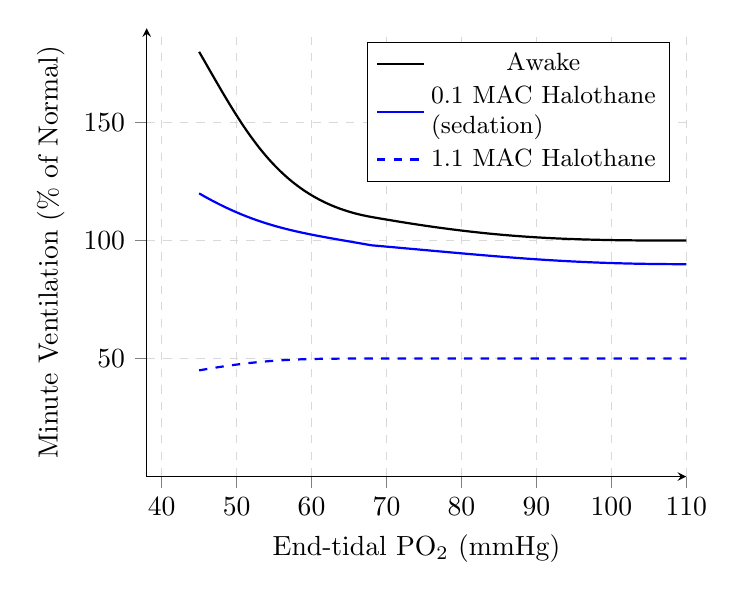
\begin{tikzpicture}
		\begin{axis}[
			axis lines=middle,
			ymin = 0,
			ymax = 190,
			xmin = 38,
			xmax= 110,
			grid = major,
			grid style={dashed, gray!30},
			ylabel near ticks,
			xlabel near ticks,
			xlabel= End-tidal PO$_2$ (mmHg),
			ylabel=Minute Ventilation (\% of Normal),
			tick align=outside,
			legend pos= north east,
			legend style={font=\small, cells={align=left}}]
	
		\draw [black, thick] (45, 180) to [out = 300, in = 170] (68,110) to [out = 350, in = 180] (110,100);
		\draw [blue, thick] (45, 120) to [out = 330, in = 170] (68,98) to [out = 355, in = 180] (110,90);
		\draw [blue, thick, dashed] (45, 45) to [out = 10, in = 180] (68,50) to [out = 0, in = 180] (110,50);

		\addlegendimage{black, thick};
		\addlegendentry{Awake};
		\addlegendimage{blue, thick};
		\addlegendentry{0.1 MAC Halothane \\ (sedation)};
		\addlegendimage{blue, dashed, thick};
		\addlegendentry{1.1 MAC Halothane};

		\end{axis}
	\end{tikzpicture} 
\end{document}